\documentclass[11pt]{article}
\usepackage[margin=1.0in]{geometry}
\usepackage{graphicx}
\usepackage[pdftex]{hyperref}
\usepackage{wrapfig}
\usepackage{float}

\title{User Empathy Reflection}
\author{Jonathan "Sumner" Evans}
\date{Section U. \today}

\begin{document}
\maketitle

\section{Introduction} % TODO: Finish Intro
Food deserts are areas that lack access to affordable fruits, vegetables, whole grains, lowfat milk,
and other foods that make up the full range of a healthy diet \cite{cdc}. 

\section{Anticipated Bugs}
Before embarking on the User Empathy Experience with my team, I compiled a list of "bugs" that I
anticipated my team would encounter while in the food desert. Below is that list with an explanation
of each item:

\begin{itemize}
    \item \textbf{Difficulty finding enough quality fruits and vegetables.} One of the challenges of
        living in a food desert is that it is difficult to find affordable fruits and vegetables
        \cite{cdc}. Because of this, I anticipated that it would be difficult for my team to find
        enough quality fruits and vegetables.

    \item \textbf{Difficulty staying under the SNAP budget.} For this assignment, we attempted to
        simulate a family's experience in a food desert. One way we did this was by challenging
        ourselves to buy all of the food for our meal on a SNAP budget. SNAP is a USDA program which
        provides food assistance for low-income individuals and families \cite{usda}. SNAP provides
        approximately \$4.32 per person per day to its beneficiaries \cite{cbpp}. For a family of
        five, that works out to be \$21.15 for the entire family for the day. I anticipated that we
        would have problems staying under that budget. I made this judgment by looking at the
        receipt from a recent grocery trip where my family spent about \$177.00. Dividing this
        number out between the four people in my family, would result in about \$69.00 per person.
        \$69.00 divided by \$4.32 is about $16$ meaning that we would have had to live solely off
        of the food we bought during that shopping trip for $16$ days. In my family, it is common to
        buy groceries approximately once a week so we would have definitely not have been able to
        eat well for all $16$ days.

    \item \textbf{Difficulty finding stores that accept EBT.} An Electronic Benefits Transfer (EBT)
        Card is the method by which SNAP funds are distributed. EBT is not accepted at every food
        retailer so I anticipated that we might have trouble finding a retailer that accepts EBT.

    \item \textbf{Difficulty finding low-fat protein sources.} In many food deserts, fast food
        chains and convenience stores are the closest, if not only, food retailers in the area
        \cite{gallagher}. Although many of these food retailers serve forms of protein, they are
        often high in fat content. Because of this, I anticipated that it would be difficult to find
        low-fat protein sources.

    \item \textbf{Difficulty finding low-fat dairy.} Judging from my past experiences at gas station
        curb stores, high-fat dairy such as ice cream is in abundance, but low-fat dairy such as
        milk or yogurt is not as common. Since curb stores are often the only retailers of food in
        food deserts, I anticipated that it would be difficult to find such low-fat dairy.

    \item \textbf{Difficulties using public transportation.} I have used public transportation in
        many places around the world with varying degrees of success. In some cases, such as when I
        used the Tube in London, things went smoothly. Other cases, such as when I attempted to ride
        a bus in New York City, were not so successful. Despite having grown up in the Denver Metro
        area, I am not very experienced in using the public transportation so I decided to assume
        the worst case scenario. Judging from past mistakes while using public transportation, I
        thought that it would be likely that we might miss the bus, get on the wrong bus, have to
        wait a long time for the bus, or miss a connection with the Light Rail.\\
        \\
        In addition, I expected that it might be cumbersome carrying the groceries on public
        transportation. While in Boston for vacation this summer, I used the public transportation
        system to get around the city and I was often carrying a backpack. This was rather
        cumbersome at times. Therefore I expected carrying groceries to also be cumbersome.

    \item \textbf{Significant amount of time to find proper foods} I anticipated that it would take
        a significant amount of time to find the proper foods (if we were even able do to) because
        of all of the aforementioned factors.
\end{itemize}

\section{Actual Bugs}
During my teams trip to our assigned food desert, we encountered many difficulties. Some were
expected, but others were surprising. All of them gave me insight into the difficulties faced by
people living in food deserts.

\begin{itemize}
    \item \textbf{Public transportation issues.} During my team's User Empathy Experience, we
        used three types of public transportation: Light Rail, bus, and walking. We didn't fully
        succeed at any of them. The Light Rail trip from Golden to Wadsworth was uneventful. While
        on the train, I took a picture of the light rail and later sketched it [Fig. 1]. Our
        troubles began after we arrived at the Wadsworth station because we had mistimed our ride
        and the Wadsworth bus was not going to come for another quarter of an hour. We ended up
        walking one mile from Colfax to 26th Avenue. At this point, the bus had caught
        up to us and we took it from 26th to 38th. Had we waited for the bus to come to the Colfax
        stop, we would have arrived at the same time, without the mile of walking.\\
        \begin{figure}[p]
            \centering
            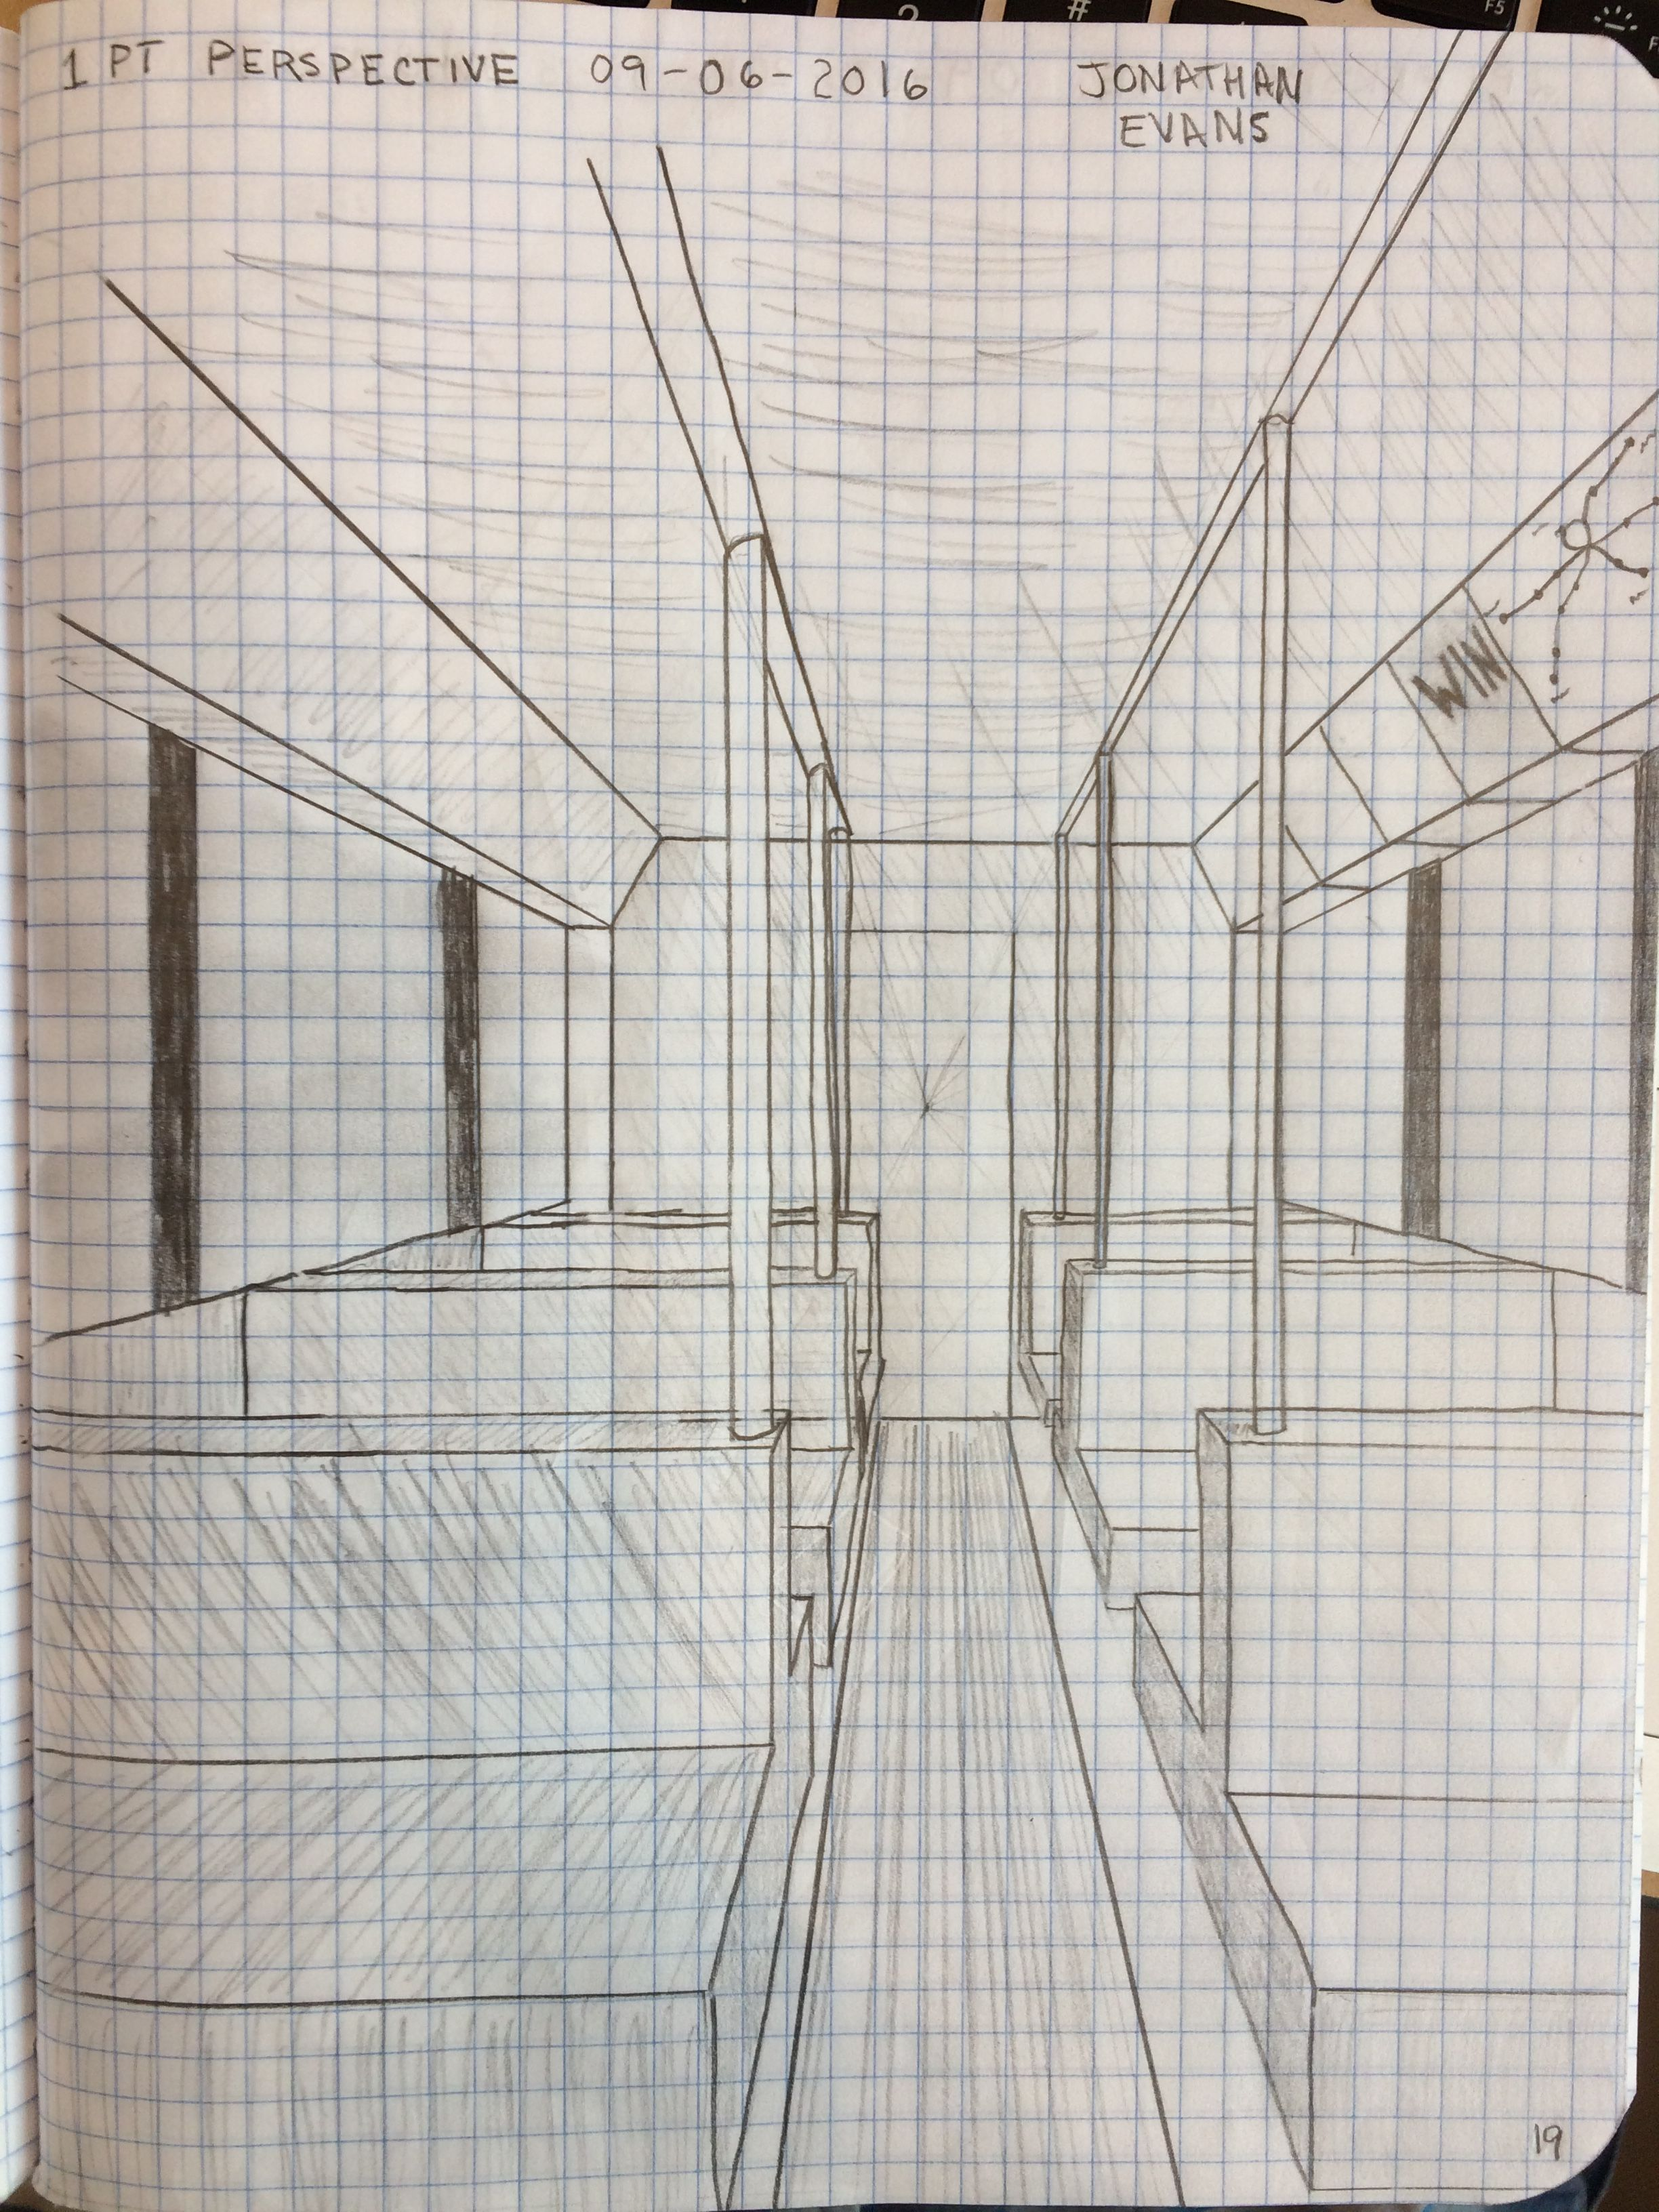
\includegraphics[width=160mm]{resources/light-rail-sketch.jpg}
            \caption{Sketch of Inside of Light Rail}
        \end{figure}
        \\
        In our food desert, there were some stretches with nice paved sidewalks, but in other
        places the sidewalks were either in poor condition or nonexistent. For example, along
        Wadsworth near the Morning Side Retirement Community, there is no paved sidewalk, it is
        merely trampled down grass and dirt. I thought that it would be difficult for some of the
        less mobile residents of the retirement community to go to the store if that was the only
        sidewalk. (When I returned on my own last Friday, I found that there are sidewalks on the
        other side of the retirement community that are in good condition, but when we were there as
        a team, we didn't find those sidewalks.)\\
        \\
        After our time in the food desert, we mistimed the bus and ended up walking $1.5$ miles from
        the food desert to the Light Rail stop at Colfax. The bus passed us about a block before we
        got to the Colfax station. As we were coming up to the Light Rail station, we saw the train
        leaving the station so we had to wait for the next train.\\
        \\
        As we walked back to the Light Rail station, I was carrying the bag of groceries. Though not
        very heavy, carrying the bag for that distance seemed to increase its weight.\\
        \\
        Overall, we were not successful in our use of public transportation. It gave me a greater
        appreciation for people who rely on public transportation for all of their transportation
        needs.

    \item \textbf{Difficulty finding quality fruits and vegetables.} We bought our food at the
        Shell curb store at 38th and Wadsworth. We found a great lack of fruits and vegetables in
        this location. There were no fresh fruits or vegetables in the store when we went as a team.
        There was a stand for bananas, but this stand was empty. When I returned on my own to the
        food desert, there was one banana in the stand. There was no shortage of fruit-flavored
        candies in the store, but no actual fruit. The closest thing to a fruit that we were able to
        find was a jar of grape jam, a highly processed derivative of a fruit. I knew that it would
        be difficult to find fruits and vegetables, but I was surprised at how sparse the selection
        was. I expected that there might be some apples or bananas consistently available but after
        two visits, it was clear that this was not the case.

    \item \textbf{Difficulty transporting perishables.} For our dairy product, we purchased some
        milk but did not account for the fact that it needed to be refrigerated. By the time we got
        back to the Mines Campus, the milk was still cool, but had noticeably heated up. If the day
        had been any warmer or if we had had to wait for a longer time between arriving on campus
        and eating our food, the milk may have been warmer and less safe.

    \item \textbf{Possible language barriers.} Our team's food desert was 

\end{itemize}

\section{Analysis}

\section{Remaining Unknowns}

\section{Summary and Conclusion}

\pagebreak
\begin{thebibliography}{9}
    \bibitem{cdc}
    Centers for Disease Control and Prevention (2012).
    \textit{A Look Inside Food Deserts} [Online].
    Available: \url{http://www.cdc.gov/features/FoodDeserts/index.html}.
    [Accessed 11-Sep-2016].

    \bibitem{usda}
    United States Department of Agriculture (2016).
    \textit{Supplemental Nutrition Assistance Program (SNAP)} [Online].
    Available: \url{http://www.fns.usda.gov/snap/supplemental-nutrition-assistance-program-snap}.
    [Accessed 11-Sep-2016].

    \bibitem{cbpp}
    Center of Budget and Policy Priorities (2015).
    \textit{A Quick Guide to SNAP Eligibility and Benefits} [Online].
    Available: \url{http://www.cbpp.org/research/a-quick-guide-to-snap-eligibility-and-benefits}.
    [Accessed 11-Sep-2016].

    \bibitem{gallagher}
    Mari Gallagher Research and Consulting Group (2014).
    \textit{Food Desert Balance Community Fact Sheet} [Oneline].
    Available:
    \url{http://www.marigallagher.com/site_media/dynamic/project_files/Food-Desert-and-Food-Balance-Fact-Sheet.pdf}
    [Accessed 12-Sept-2016].

\end{thebibliography}
\end{document}
